%%%%%%%%%%%%%%%%%%%%%%%%%%%%%%%%%%%%%%%%%%%%%%%%%%%%%%%%%%%%%%%%%%%%%
% LaTeX Template: Project Titlepage Modified (v 0.1) by rcx
%
% Original Source: http://www.howtotex.com
% Date: February 2014
% 
% This is a title page template which be used for articles & reports.
% 
% This is the modified version of the original Latex template from
% aforementioned website.
% 
%%%%%%%%%%%%%%%%%%%%%%%%%%%%%%%%%%%%%%%%%%%%%%%%%%%%%%%%%%%%%%%%%%%%%%

\documentclass[12pt]{report}
\usepackage[a4paper]{geometry}
\usepackage[myheadings]{fullpage}
\usepackage{fancyhdr}
\usepackage{lastpage}
\usepackage{graphicx, wrapfig, subcaption, setspace, booktabs}
\usepackage[T1]{fontenc}
\usepackage[font=small, labelfont=bf]{caption}
\usepackage{fourier}
\usepackage[protrusion=true, expansion=true]{microtype}
\usepackage[english]{babel}
\usepackage{sectsty}
\usepackage{url, lipsum}
\usepackage{tgbonum}
\usepackage{hyperref}
\usepackage{xcolor}

\newcommand{\HRule}[1]{\rule{\linewidth}{#1}}
\onehalfspacing
\setcounter{tocdepth}{5}
\setcounter{secnumdepth}{5}



%-------------------------------------------------------------------------------
% HEADER & FOOTER
%-------------------------------------------------------------------------------
%\pagestyle{fancy}
%\fancyhf{}
%\setlength\headheight{15pt}
%\fancyhead[L]{Student ID: 1034511}
%\fancyhead[R]{Anglia Ruskin University}
%\fancyfoot[R]{Page \thepage\ of \pageref{LastPage}}
%-------------------------------------------------------------------------------
% TITLE PAGE
%-------------------------------------------------------------------------------
\pagestyle{fancy}
\fancyhf{}
\setlength\headheight{15pt}
\fancyhead[L]{Group 27}
\fancyhead[R]{University of Maryland}
\fancyfoot[R]{Page \thepage\ of \pageref{LastPage}}


\begin{document}
{\fontfamily{cmr}\selectfont
\title{ \textsc{ENPM 673}
\normalsize \textsc{}
		\\ [2.0cm]
		\HRule{0.5pt} \\
		\LARGE \textbf{\uppercase{Project 2}
		\HRule{2pt} \\ [0.5cm]
		\normalsize \today \vspace*{5\baselineskip}}
		}

\date{}

\author{
		Markose Jacob 117000269 \\ 
		Karan Sutradha 117037272\\ 
		Trevian Jenkins 116781381\\ 
	    University of Maryland \\
		 }

\maketitle

\newpage

%-------------------------------------------------------------------------------
% Section title formatting
\sectionfont{\scshape}
%-------------------------------------------------------------------------------

%-------------------------------------------------------------------------------
% BODY
%-------------------------------------------------------------------------------

\section*{Problem 1}
The aim was to improve the quality of the video sequence.  The first step was to convert the video to frames and then apply a filter to reduce the noise in the video. After application of a Gaussian filter, we knew that the video was dark, and we must improve the brightness and contrast in order to have a higher-quality video. So, the next step was to perform a histogram equalization. \newline
\subsection*{Histogram Equalization}
\begin{figure}[h!]
    \centering
    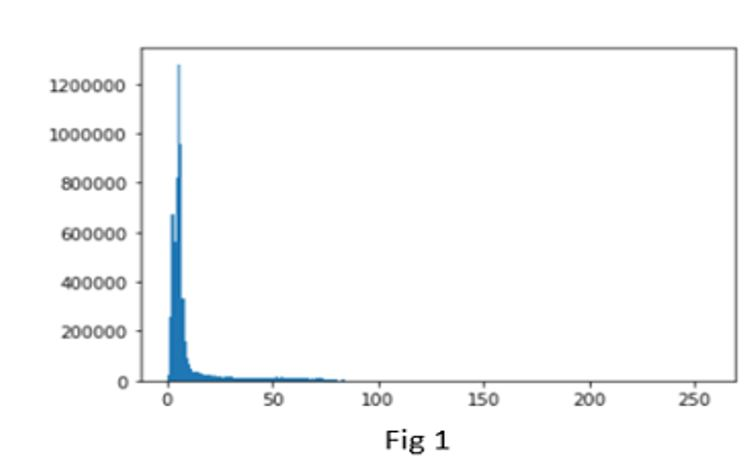
\includegraphics[scale=0.4]{Capture1.JPG}
    \caption{Original video histogram}
    \label{fig:my_label2}
\end{figure}
\begin{figure}[h!]
    \centering
    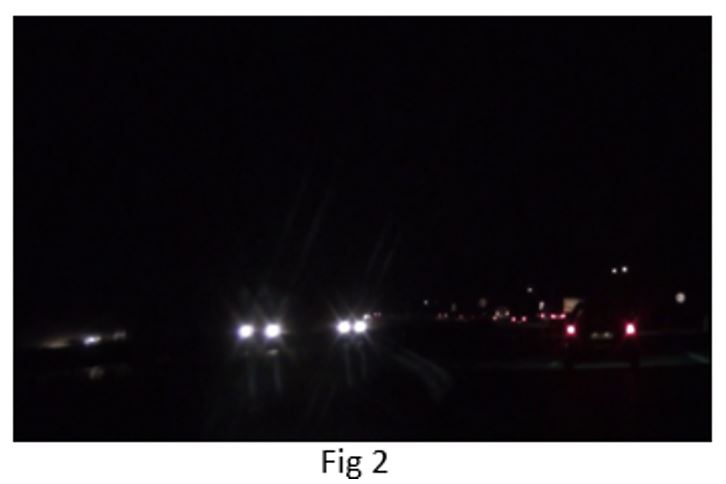
\includegraphics[scale=0.4]{Capture2.JPG}
    \caption{Original video screen shot}
    \label{fig:my_label2}
\end{figure}


From the plot in Fig 1, we see that the histogram lies primarily in a darker region.  We need a uniform distribution of both the dark and bright regions. We must transform the histogram of the image so that it achieves this even distribution.  Histogram equalization improves the contrast and brightness of the image. \newline

\subsection*{Grayscale Image - Histogram Equalization} 

First the frames were read and converted into grayscale.  We normalized the video frame using histogram equalization. The idea was to spread out the histogram so that it makes full use of the dynamic range of the image. We got a normalized graph, but the video was rather noisy. \newline
\begin{figure}[h!]
    \centering
    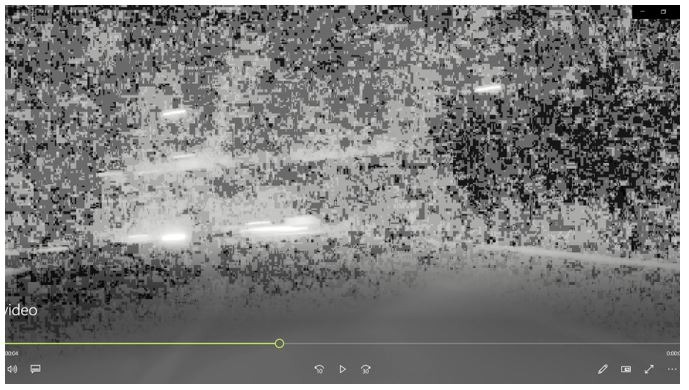
\includegraphics[scale=0.4]{Capture3.JPG}
    \caption{Gray scale Histogram Equalization video output screenshot}
    \label{fig:my_label2}
\end{figure}
\begin{figure}[h!]
    \centering
    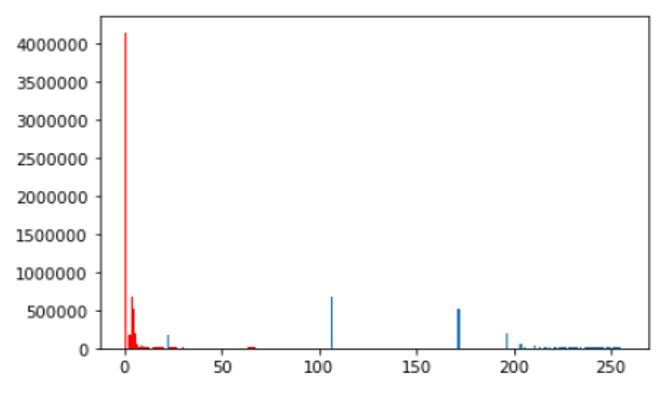
\includegraphics[scale=0.4]{Capture4.JPG}
    \caption{Gray scale video histogram equalization}
    \label{fig:my_label2}
\end{figure}


\subsection*{Canny Edge Detection – Histogram Equalization} 

In both the above cases the video output was noisy, so we tried application of canny edge detection and then applied histogram. We still got an output with noise.\newline

\subsection*{Color Image - Histogram Equalization}

Since the video was dark with color pixels (RGB) present, we separated the images into green, blue and red channels, applied a histogram equalization individually on these channels, and merged the image back. We again got a normalized graph, but the video was with full of noise. \newline

\begin{figure}[h!]
    \centering
    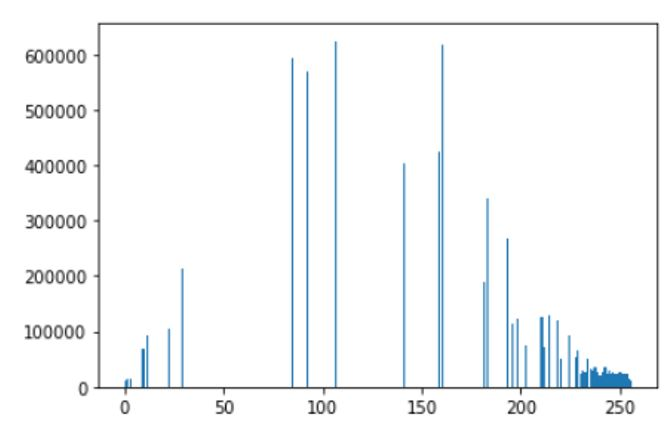
\includegraphics[scale=0.4]{Capture5.JPG}
    \caption{Colour video Histogram Equalization}
    \label{fig:my_label2}
\end{figure}
\begin{figure}[h!]
    \centering
    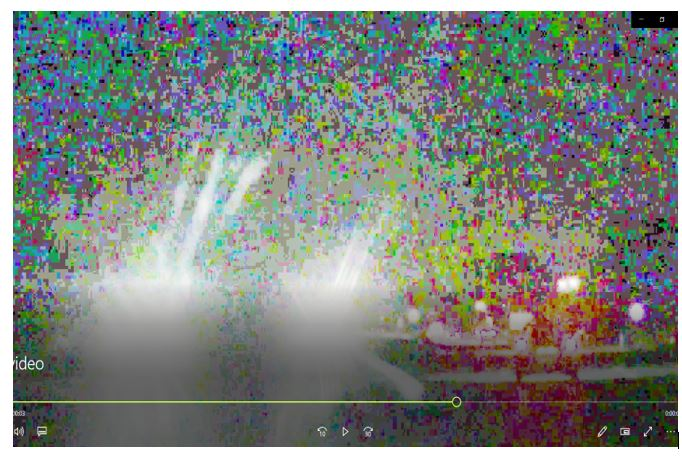
\includegraphics[scale=0.4]{Capture6.JPG}
    \caption{Colour Video Screenshot}
    \label{fig:my_label2}
\end{figure}





\subsection*{Gamma-Correction} 
To apply gamma correction, the image pixel intensity is to be scaled from the limit of [0, 255] to [0, 1]. By applying the equation $O = I^{(1/G)}$ we get the gamma-corrected image. \newline
‘I’ is the input image and ‘G’ is the gamma value. The output image ‘O’ is then scaled back to the range [0, 255]. \newline
Gamma values less than 1.0 will shift the image towards the darker region and gamma value greater than than 1.0 will make the image brighter. A gamma value of 1.0 will have no effect on the input image.
We had the best output after applying gamma correction. \newline
In our program we tried using different gamma values and found that the value of 3.0 gives the best result. \newline 
We concluded that gamma correction gives the best output in order to make the image brighter and hence discarded our previous attempts to in making the video brighter. \newline

\begin{figure}[h!]
    \centering
    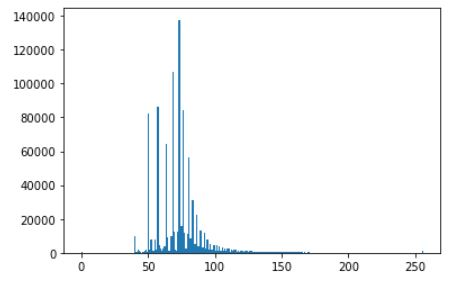
\includegraphics[scale=0.65]{Capture7.JPG}
    \caption{Gamma Correction Histogram}
    \label{fig:my_label2}
\end{figure}
\begin{figure}[h!]
    \centering
    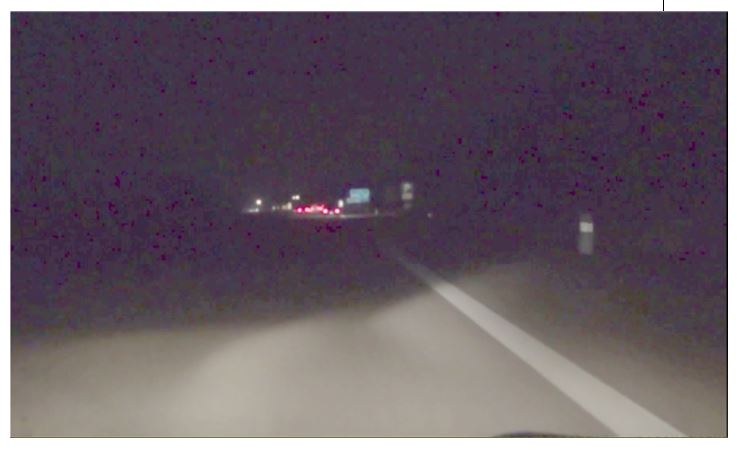
\includegraphics[scale=0.4]{Capture8.JPG}
    \caption{Gamma Correction Video Screenshot}
    \label{fig:my_label2}
\end{figure}
\vspace{50mm}



\newline

\section*{Problem 2}
The pipeline we followed to solve this problem is described in this section.
\subsection*{Undistort the image}
By using the camera matrix and distortion coefficients we first undistorted the image.
\begin{figure}[h!]
    \centering
    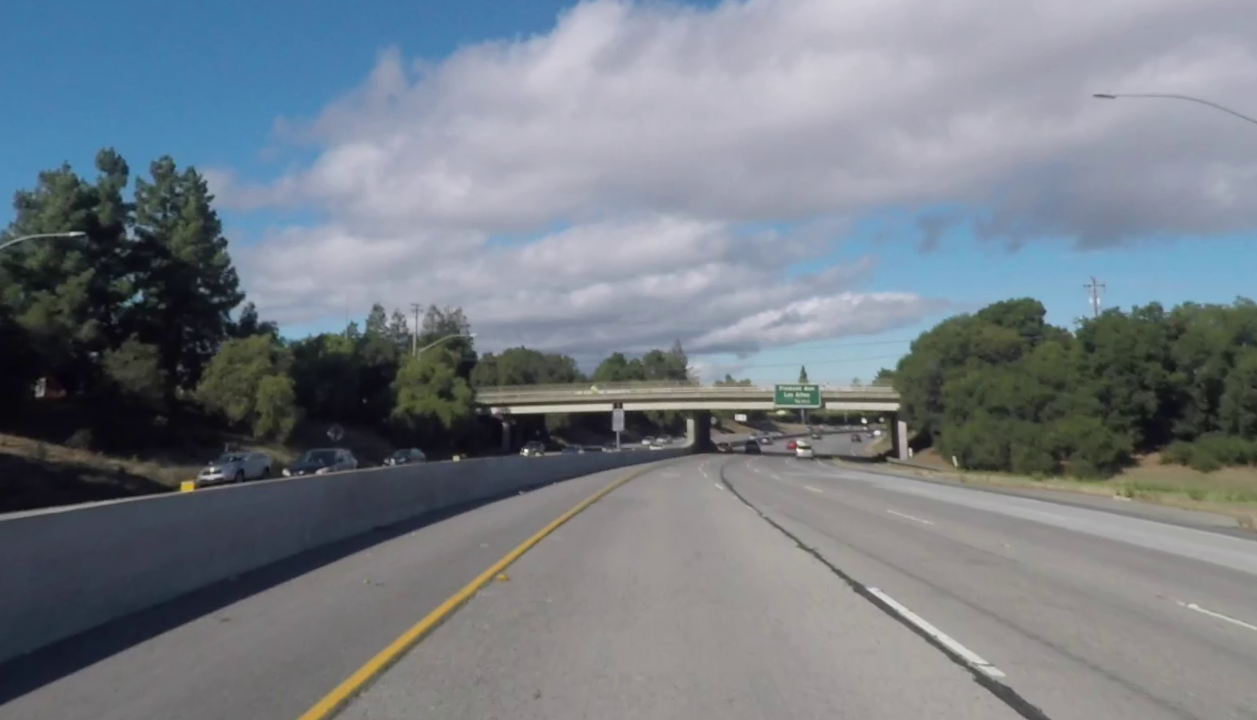
\includegraphics[scale=0.2]{undistort__01.png}
    \caption{Undistored image}
    \label{fig:my_label2}
\end{figure}
\subsection*{Finding yellow regions which correspond to lanes}
We first isolated the yellow regions in the image based on the hue and value, using erosion and dilation to smooth the regions for edge and line detection.
\begin{figure}[h!]
    \centering
    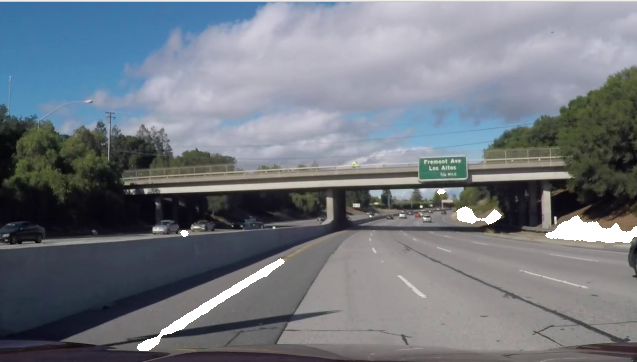
\includegraphics[scale=0.4]{yellow__01.png}
    \caption{Emphasized Yellow Region}
    \label{fig:my_label2}
\end{figure}
\subsection*{Finding white regions which correspond to lanes}
To find the white regions from the masked image we first convert the image to gray scale and use Gaussian and bilateral filters to remove noise, followed be a threshold application.  Erosion and dilation are performed again to encompass the lines of interest, and the resulting mask is applied to the original image.  This step would find white lines on both sides of the road in case there were no yellow lines.
\begin{figure}[h!]
    \centering
    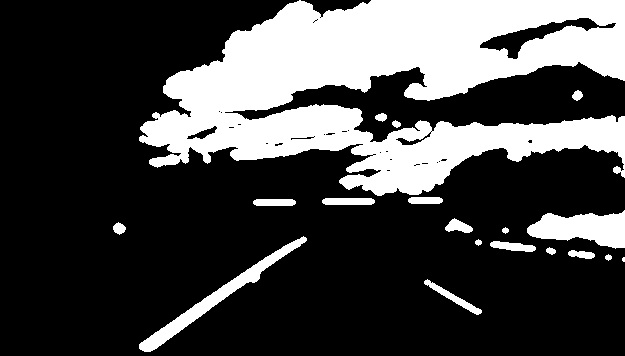
\includegraphics[scale=0.4]{white__01__01.png}
    \caption{white regions}
    \label{fig:my_label2}
\end{figure}
\subsection*{Finding gray regions which correspond to surface of the road}
The gray region of the image was found similarly to the yellow region.  We looked for areas with moderate intensity and low saturation, corresponding to the road.  We dilated this area to encompass the region of interest so that background elements (sky, trees, cars, etc.) would be excluded while our lane lines would be preserved.  By dilating and inverting this region and using a bitwise-AND operation, we excluded the middle of the road from land detection, overcoming the challenge of distinguishing cracks in the road from lanes, as seen in the challenge video.
\begin{figure}[h!]
    \centering
    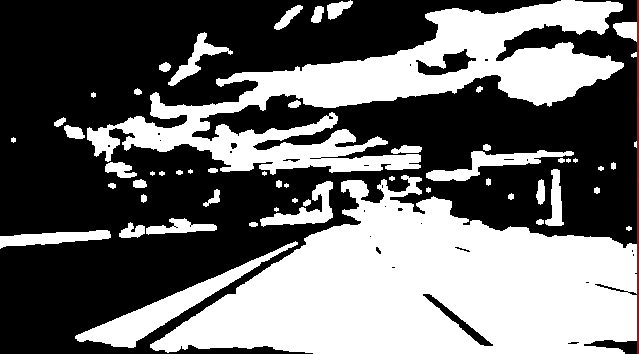
\includegraphics[scale=0.4]{gray__01.png}
    \caption{gray regions}
    \label{fig:my_label2}
\end{figure}
\subsection*{Edge detection}
We then used canny edge detection to find the edges. After edge detection we cropped the image to get rid of the top half where there are no lanes present, and we applied the mask described in the previous section.
\begin{figure}[h!]
    \centering
    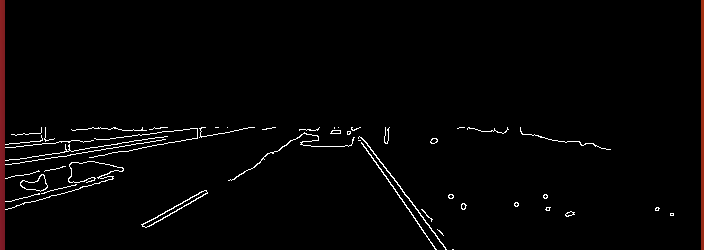
\includegraphics[scale=0.4]{canny__01.png}
    \caption{Edge detection}
    \label{fig:my_label2}
\end{figure}
\subsection*{Hough lines}
We then used the Hough transform to identify lines within the image.  The resulting lines in the Hough transform were separated into two groups based off the slope of each line.  Lines with a low absolute slope were excluded, as they more likely arose from background elements.  After averaging the slope and y-intercept of each group, we were able to distinguish two major lines corresponding to our lane edges.

\subsection*{Overlay}

We found the horizon based off the proportion width of the gray region of the image to place the cutoff for drawing the lane.  The lane lines determined from the Hough transform were used to project the lanes onto the original image.

\subsection*{Turn Prediction }
Using the four vertices of the Hough lines, we calculated the homography and unwarped the image.  Using the yellow and white masks generated previously, we fit a 2nd-order polynomial equation to each line.  The sign of the highest-order coefficient determined the 2nd derivative of the line, which in turn determined if the lane was turning, and which direction.  If the sign of this coefficient was the same for both sides, then the lane was indeed turning.  A positive 2nd derivative corresponded to a right turn, and a negative sign corresponded with the left.

\begin{figure}[h!]
    \centering
    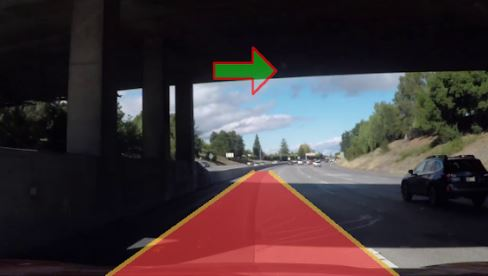
\includegraphics[scale=1.0]{TurnPrediction.JPG}
    \caption{Turn prediction demonstration}
    \label{fig:my_label2}
\end{figure}

\section*{Video Output}
The video output for problem 1  can be found in the link below :  \newline
\vspace{3mm}
\url{https://drive.google.com/file/d/1xVnW3HPCQgHPMpyd9vPtDBQxUYa2TQEI/view?usp=sharing} \newline\vspace{3mm}
The video output for problem 2  can be found in the link below :  \newline
\vspace{3mm}
Day Drive: \url{https://drive.google.com/open?id=1rCX3lqPK5dk8fWKKc79EiC4bV_fdv5ed}\newline
Challenge: \url{https://drive.google.com/open?id=10ieWuzF8WZSwEkLLht0K0qhOLmLJqB8c}\newline
Extra example: \url{https://drive.google.com/open?id=1CQWk95V5ops7hOQCqZ205Dq00V4p3SmG}\newline\vspace{3mm}
We recommend to use VLC for playing the videos. \newline 

{\fontsize{14pt}{16.8pt}\selectfont \textbf{NOTE: }\par}\par

To run the code you need to follow the README file.\par



\section*{Additional}
Additionally we also executed our code on different videos and found the results to be satisfactory.
\begin{figure}[h!]
    \centering
    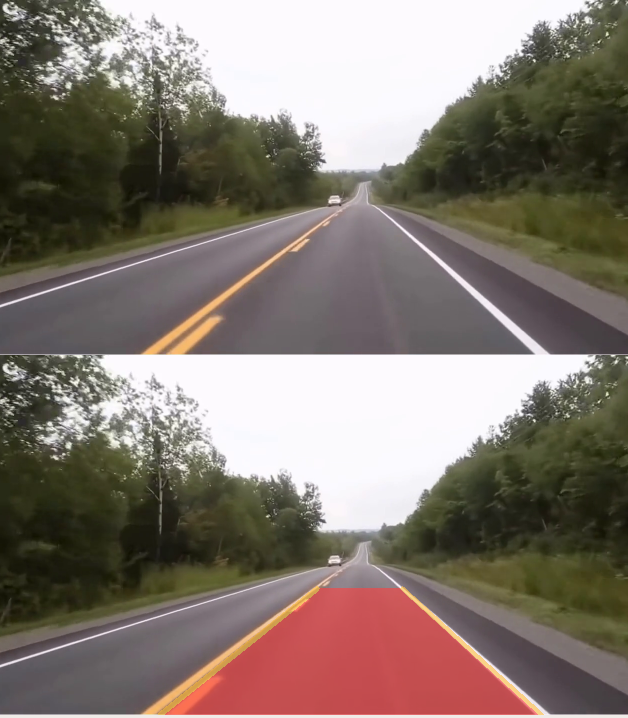
\includegraphics[scale=0.4]{video1__01.png}
    \caption{Video 1}
    \label{fig:my_label2}
\end{figure}

\begin{figure}[h!]
    \centering
    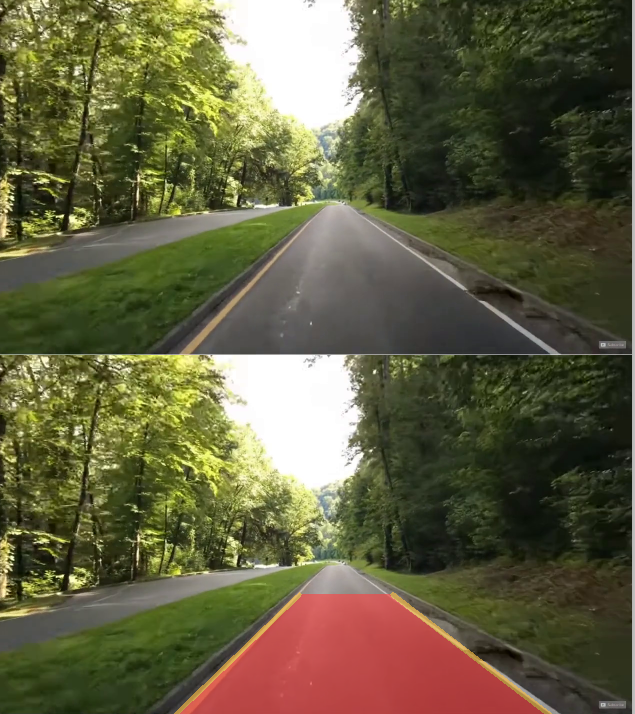
\includegraphics[scale=0.4]{video6__01.png}
    \caption{Video 2}
    \label{fig:my_label2}
\end{figure}

\begin{figure}[h!]
    \centering
    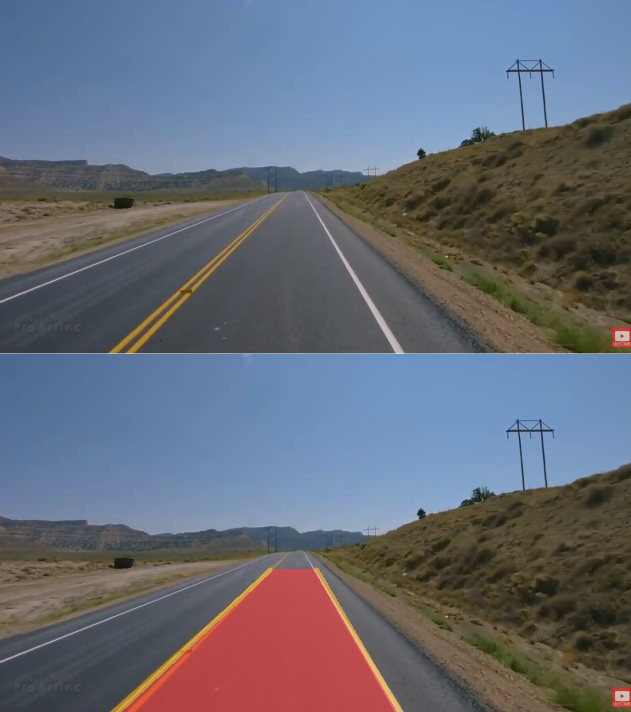
\includegraphics[scale=0.4]{video7__01.png}
    \caption{Video 3}
    \label{fig:my_label2}
\end{figure}
\newpage

}
\end{document}

%-------------------------------------------------------------------------------
% SNIPPETS
%-------------------------------------------------------------------------------

%\begin{figure}[!ht]
%	\centering
%	\includegraphics[width=0.8\textwidth]{file_name}
%	\caption{}
%	\centering
%	\label{label:file_name}
%\end{figure}

%\begin{figure}[!ht]
%	\centering
%	\includegraphics[width=0.8\textwidth]{graph}
%	\caption{Blood pressure ranges and associated level of hypertension (American Heart Association, 2013).}
%	\centering
%	\label{label:graph}
%\end{figure}

%\begin{wrapfigure}{r}{0.30\textwidth}
%	\vspace{-40pt}
%	\begin{center}
%		\includegraphics[width=0.29\textwidth]{file_name}
%	\end{center}
%	\vspace{-20pt}
%	\caption{}
%	\label{label:file_name}
%\end{wrapfigure}

%\begin{wrapfigure}{r}{0.45\textwidth}
%	\begin{center}
%		\includegraphics[width=0.29\textwidth]{manometer}
%	\end{center}
%	\caption{Aneroid sphygmomanometer with stethoscope (Medicalexpo, 2012).}
%	\label{label:manometer}
%\end{wrapfigure}

%\begin{table}[!ht]\footnotesize
%	\centering
%	\begin{tabular}{cccccc}
%	\toprule
%	\multicolumn{2}{c} {Pearson's correlation test} & \multicolumn{4}{c} {Independent t-test} \\
%	\midrule	
%	\multicolumn{2}{c} {Gender} & \multicolumn{2}{c} {Activity level} & \multicolumn{2}{c} {Gender} \\
%	\midrule
%	Males & Females & 1st level & 6th level & Males & Females \\
%	\midrule
%	\multicolumn{2}{c} {BMI vs. SP} & \multicolumn{2}{c} {Systolic pressure} & \multicolumn{2}{c} {Systolic Pressure} \\
%	\multicolumn{2}{c} {BMI vs. DP} & \multicolumn{2}{c} {Diastolic pressure} & \multicolumn{2}{c} {Diastolic pressure} \\
%	\multicolumn{2}{c} {BMI vs. MAP} & \multicolumn{2}{c} {MAP} & \multicolumn{2}{c} {MAP} \\
%	\multicolumn{2}{c} {W:H ratio vs. SP} & \multicolumn{2}{c} {BMI} & \multicolumn{2}{c} {BMI} \\
%	\multicolumn{2}{c} {W:H ratio vs. DP} & \multicolumn{2}{c} {W:H ratio} & \multicolumn{2}{c} {W:H ratio} \\
%	\multicolumn{2}{c} {W:H ratio vs. MAP} & \multicolumn{2}{c} {\% Body fat} & \multicolumn{2}{c} {\% Body fat} \\
%	\multicolumn{2}{c} {} & \multicolumn{2}{c} {Height} & \multicolumn{2}{c} {Height} \\
%	\multicolumn{2}{c} {} & \multicolumn{2}{c} {Weight} & \multicolumn{2}{c} {Weight} \\
%	\multicolumn{2}{c} {} & \multicolumn{2}{c} {Heart rate} & \multicolumn{2}{c} {Heart rate} \\
%	\bottomrule
%	\end{tabular}
%	\caption{Parameters that were analysed and related statistical test performed for current study. BMI - body mass index; SP - systolic pressure; DP - diastolic pressure; MAP - mean arterial pressure; W:H ratio - waist to hip ratio.}
%	\label{label:tests}
%\end{table}%\documentclass{article}
%\usepackage[utf8]{inputenc}

%\title{Weekly Report template}
%\author{gandhalijuvekar }
%\date{January 2019}

%\begin{document}

%\maketitle

%\section{Introduction}

%\end{document}
